\documentclass[a4paper, 11pt]{article}

\usepackage{xcolor}
\input{/home/aroquemaurel/cours/templates/templates/couleurs.tex}
\usepackage{lmodern}
\usepackage[utf8]{inputenc}
\usepackage[T1]{fontenc} \usepackage[francais]{babel}
\usepackage[top=1.7cm, bottom=1.7cm, left=2.5cm, right=2.5cm]{geometry}
\usepackage{verbatim}
\usepackage{tikz} %Vectoriel
\usepackage{pgfplots}
\usepackage{listings}
\usepackage{fancyhdr}
\usepackage{multido}
\usepackage{amssymb}
\usepackage{multicol}
\usepackage{float}
\usepackage[urlbordercolor={1 1 1}, linkbordercolor={1 1 1}, linkcolor=vert1, urlcolor=bleu, colorlinks=true]{hyperref}

\newcommand{\titre}{Plaquage de textures en lancer de rayons}
\newcommand{\numero}{3}
\newcommand{\typeDoc}{DM}
\newcommand{\module}{Outils Informatiques pour le Multimédia}
\newcommand{\sigle}{OIM}
\newcommand{\semestre}{7}
\newcommand{\auteur}{Antoine de \bsc{Roquemaurel} (G1.1)}

\input{/home/aroquemaurel/cours/templates/templates/classroomsTemplates/l3/tddm.tex}
\input{/home/aroquemaurel/cours/templates/templates/listings.tex} %prise en charge du langage C 
\input{/home/aroquemaurel/cours/templates/templates/classroomsTemplates/l3/remarquesExempleAttention.tex}
\input{/home/aroquemaurel/cours/templates/templates/polices.tex}
\input{/home/aroquemaurel/cours/templates/templates/affichageChapitre.tex}
\makeatother

\begin{document}
	\maketitle
	\section{Avant-propos}
	L'archive que vous avez obtenu sur Moodle contient plusieurs fichiers organisés comme suit : 
	\begin{description}
		\item[\texttt{src/}] Contient uniquement les fichiers modifiés, c'est-à-dire \texttt{main.cpp} et \texttt{texturefetch.cpp}.
		\item[\texttt{report\_AntoinedeRoquemaurel.pdf}] Le présent rapport que vous êtes en train de lire
	\end{description}
	\section{Opérateur \texttt{getTextel()}}
	Une fois les textures intégrés, on peut observer un effet << d'escalier >> sur le quadrillage de l'image, principalement au premier plan, comme le montre la
	figure \ref{fig:fig1}. 

	\begin{figure}[H]
		\centering
		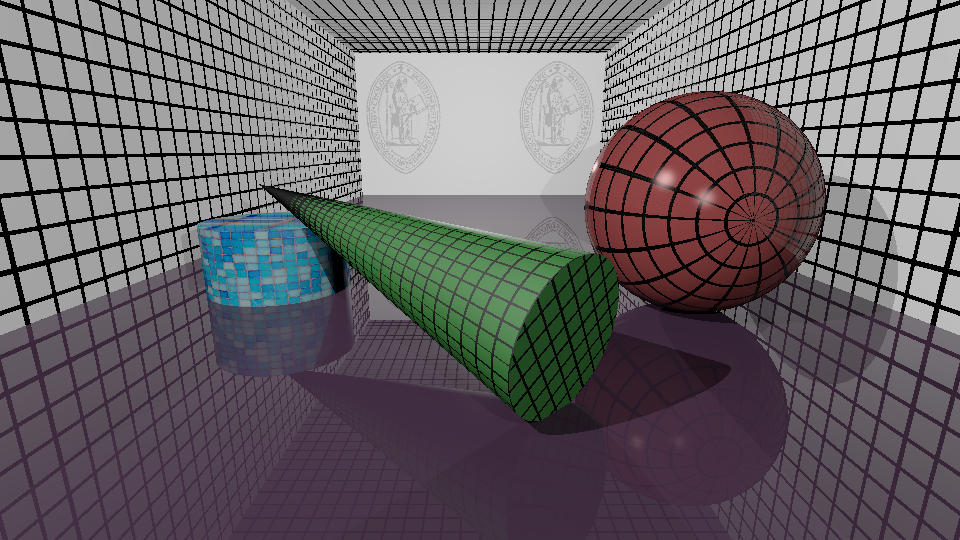
\includegraphics[width=12cm]{1-monimage.png}
		\caption{Image obtenue après le développement de \texttt{getTextel()}}
		\label{fig:fig1}
	\end{figure}
	Cela vient du fait que nous essayons d'intégrer une texture 2D sur des figures 3D. Afin de bien représenter une profondeur sur nos textures 2D, nous les
	avons déformés afin que sa taille en premier plan soit plus grande que la taille en arrière plan. C'est cette transformation qui créer un effet de crênelage
	sur le devant de la scène.
	\section{Opérateur d'interpolation linéaire pour l'accès à un élément de texture}
	\begin{figure}[H]
		\centering
		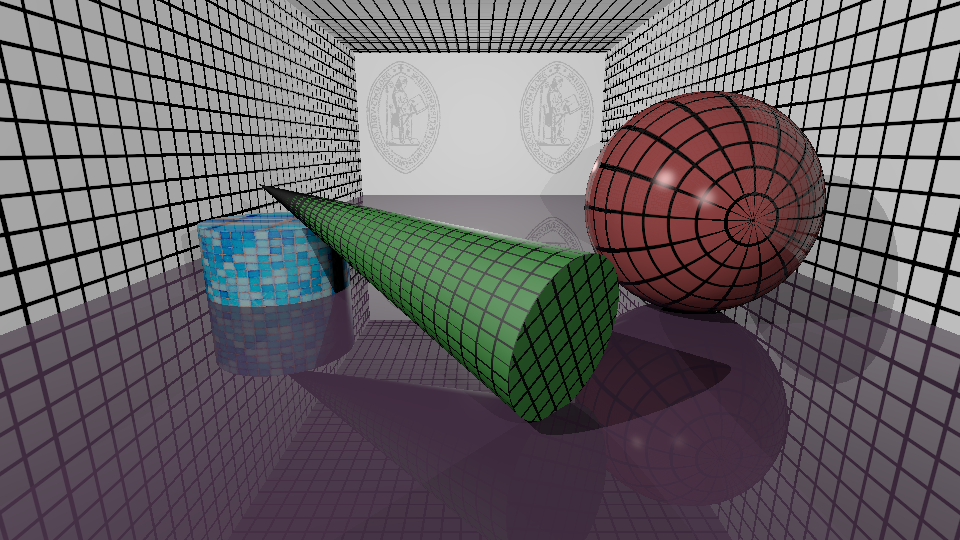
\includegraphics[width=12cm]{2-monimage.png}
		\caption{Image obtenue après le développement de \texttt{interpolateTexture()}}
		\label{fig:fig1}
	\end{figure}
	\section{Opérateur d'intégration pour le filtrage de texture}
	\begin{figure}[H]
		\centering
		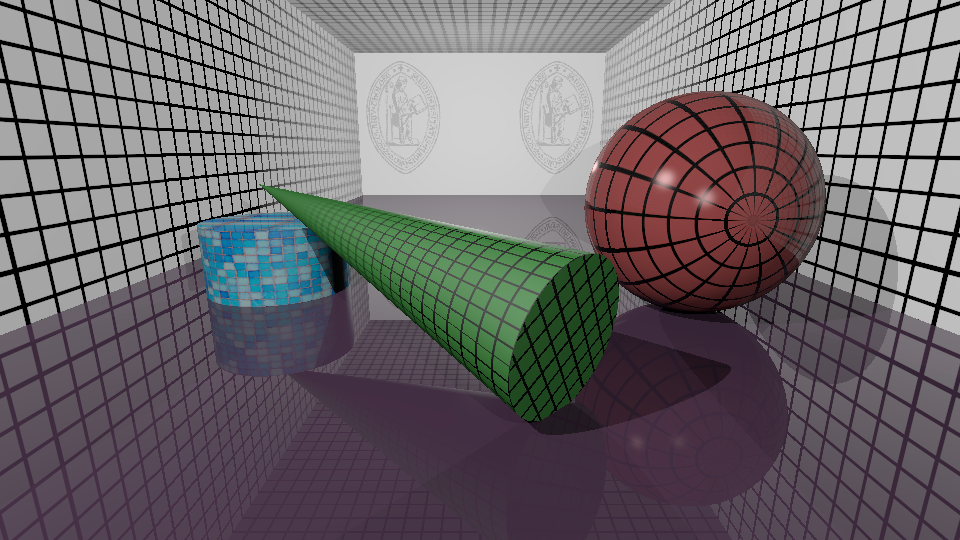
\includegraphics[width=12cm]{3-monimage.png}
		\caption{Image obtenue après le développement de \texttt{integrateTexture()}}
		\label{fig:fig1}
	\end{figure}
	\section{Opérateur de pré-filtrage de texture}
	\section{Analyse et estimation des limites des techniques de filtrage implantées}

\end{document}
